
%abstract
%Экспериментально исследовано формирование вихревого течения в сосуде с жидкостью, совершающем гармонические колебания в вертикальном направлении. Установлено, что в цилиндрическом сосуде вихревого течения не наблюдается до тех пор, пока амплитуда колебаний не превысит порогового значения, при котором развивается параметрическая неустойчивость Фарадея и на поверхности появляются азимутальные моды. В квадратном сосуде и в цилиндрическом сосуде с нарушенной симметрией вихри наблюдаются при амплитудах ниже порога параметрической неустойчивости. Предполагается, что формирование вихревого течения обусловлено взаимодействием распространяющихся под углом друг к другу поверхностных волн.


\chapter{Формирование вихревого течения капиллярными волнами на поверхности жидкости} \label{chapt3}

% Недавно появились работы, в которых докладывалось, что при возбуждении поверхности жидкости неустойчивостью Фарадея помимо волновой структуры возникает вихревое течение. Таким образом к волновой системе добавляются степени свободы связанные с вихревым движение, что может привести к перераспределению энергии и поменять свойства системы. В этой главе представлены экспериментальные и теоретические результаты изучения возникновения вихревых структур в волновых системах при накачке системы вертикальными периодическими колебаниями.
Не смотря на то, что было сделано немало работ \cite{VonKameke2011, Francois2014, Francois2013}, в которых исследованы статистические свойства турбулентной системы вихрей, возникших в результате неустойчивости Фарадея, детального исследования механизма генерации вихревого движения при развитии поверхностной неустойчивости сделано не было. В данной главе приведены результаты изучения процессов генерации вихревого движения капиллярными волнами при различных условиях возбуждения
% исследованы условия возбуждения вихревых движений при вертикальной тряске экспериментальной ячейки.


\section{Экспериментальная методика}\label{sect3_2}
Закрепленный на виброплатформе сосуд цилиндрической или квадратной формы заполняли дистиллированной водой. Сторона квадратного сосуда составляла 50 мм, внутренний диаметр цилиндрического - 65 мм, глубина обоих сосудов 10 мм. Сосуд совершает гармонические колебания в вертикальном направлении с частотой $\omega_p$ и амплитудой $S$. В связанной с сосудом системе координат, на жидкость действует "фиктивная" сила тяжести с ускорением, равным сумме ускорения свободного падения $g$ и переменного ускорения сосуда $g \beta cos(\omega_p t)$, где $\beta = S \omega_p^2/g$ – безразмерная амплитуда переменного ускорения. На стенку сосуда прикреплен акселерометра, измеряющий ускорение сосуда. В главе \ref{p1_methodsExt} было показано, что в такой системе возможны два механизма рождения волн. Волны, возникающие благодаря изменению формы мениска, будут иметь относительно слабую амплитуда. А возбуждаться будут только радиальные моды.

% Один из них связан с наличием мениска у поверхности жидкости, соприкасающейся с вертикальной стенкой сосуда. Мениск, периодически меняющий свою форму в переменном поле тяжести, служит источником поверхностной волны. Для эффективного возбуждения стоячей волны частота колебаний платформы $\omega_p$ должна быть близка к резонансной частоте колебаний поверхности жидкости в сосуде $\omega_n$. В цилиндрическом сосуде этим способом возбуждаются радиальные моды колебаний поверхности жидкости, которые описываются функцией Бесселя первого рода:

%\begin{equation}
% %\label{eq:disperCap}
%\eta(r, t) = \eta_0 cos(\omega_n t) J_0(k_n r)
%\end{equation}
%
%где n – номер резонанса, $k_n$ и $\omega_n$ – волновое число и частота моды, $\eta_0$ – амплитуда колебаний поверхности жидкости в центре сосуда. В квадратном сосуде плоские волны, распространяющиеся перпендикулярно от каждой стенки, образуют пару стоячих волн:
%
%\begin{equation}
% %\label{eq:disperCap}
%\eta(x, y, t) = \eta_x cos(\omega_n t) cos(k_n x) + \eta_y cos(\omega_n t) cos(k_n y) 
%\end{equation}
%
%Связь частоты и волнового числа определяется дисперсионным соотношением, в которое входят поверхностное натяжение $\sigma$ и плотность $\rho$ жидкости, а также глубина $h$ слоя \cite{land}
%
%%\begin{equation}
%
%% \label{eq:disper1}
%%\omega^2 = (gk + \sigma/\rho k^3)tanh(kh),
%
%%\end{equation}
%
%Другой механизм возбуждения волн связан с параметрической неустойчивостью плоской поверхности жидкости в переменном поле тяжести. Для наблюдения параметрического резонанса частота вынужденных колебаний сосуда $\omega_p$ должна быть в два раза больше частоты резонансной моды $\omega_n$. Из-за наличия затухания поверхностных волн этот механизм в отличие от предыдущего является пороговым: усиления волны не происходит, пока амплитуда переменного ускорения не превысит критического значения $\beta_c$. Величина порога оказывается больше, если частота колебаний сосуда отличается от удвоенной резонансной частоты. 
При параметрическом же возбуждении поверхностных волн в цилиндрическом сосуде, кроме радиальных мод (\ref{eq:Bessel}), также могут возбуждаться и азимутальные моды.
%
%\begin{equation}
% %\label{eq:disperCap}
%\eta(r, \phi, t) = \eta_0 cos(\omega_n t) J_0(k_n r) cos(m \phi)
%\end{equation}
%
%Допустимые значения волновых чисел здесь определяются из условия отсутствия протекания жидкости через вертикальную стенку сосуда, $k_{n, m} = \mu_n^{(m)}/R$
%где $n$, $m$ – целые числа, $R$ – радиус сосуда, $\mu_n^{(m)}$ – корни уравнения $J'_m(x) = 0$. 
%

Для декорирования течений на поверхности в воду добавляли стеклянные сферы диаметром 50 мкм, либо порошок из полиамида PA12 со средним диаметром частиц 25–30 мкм. Плотность стеклянных сфер была немного меньше плотности воды. Для получения изображения треков движения частиц на поверхности жидкости, частицы подсвечиваются фотовспышкой в стробоскопическом режиме и фотографируются с большой выдержкой. Для нахождения горизонтальной составляющей скорости течения жидкости поверхность с пробными частицами фотографировали с частотой около 5.5 кадра/с при длительности фотовспышки 1 мс. Поле скоростей определяли из парных изображений с помощью пакета PIVlab \cite{PIVlab, PIVlab1} для MatLab. 
Завихренность вычислялась из полученного поля скорости согласно формуле (\ref{eq:defVort}).


\section{Экспериментальные результаты и их обсуждение} \label{sect3_3} 
На рис. \ref{img:wave_rad} показана фотография поверхности воды в цилиндрическом сосуде, декорированной порошком из полиамида. При колебаниях виброплатформы на частоте 25 Гц с амплитудой ниже пороговой для данной частоты на поверхности жидкости возбуждается радиальная мода $n = 6$ с длиной волны $\lambda \approx 10$ мм. В зависимости от плотности и смачиваемости пробные частицы дрейфуют либо к узлам, либо к пучностям стоячих волн \cite{Lukaschuk2007}. На фотографии хорошо видны концентрические круги, сформированные частицами, которые собираются в узлах стоячей волны. Заметим, что на этом снимке вихревого движения не наблюдается. При постепенном увеличении амплитуды колебаний виброплатформы амплитуда колебаний поверхности жидкости плавно нарастает. При достижении некоторого значения амплитуды переменного ускорения $\beta$ наблюдается резкое усиление колебаний поверхности и возникает азимутальная мода (\ref{eq:Bessel}) с числом $m$ порядка 10. Эту амплитуду переменного ускорения принимали за пороговое значение $\beta_c$. Появление азимутальной моды сопровождается формированием вихревого движения на поверхности (рис. \ref{img:wave_az}). На фотографии отчетливо видна система из трех концентрических поясов вихрей. В каждом поясе содержится по 12 пар вихрей, вращающихся в противоположных направлениях. Наибольшие размеры имеют вихри внешнего пояса вблизи стенки сосуда. При дальнейшем увеличении амплитуды накачки возникают крупномасштабные течения, разрушающие концентрическое расположение вихрей.

\begin{figure}[ht] 
  \center
  \includegraphics [scale=1] {article3/pic_01.jpg}
  \caption{Фотография поверхности воды при колебаниях цилиндрического сосуда на частоте 25Гц с амплитудой меньшей критической для возбуждения параметрического резонанса} 
  \label{img:wave_rad}  
\end{figure}

\begin{figure}[ht] 
  \center
  \includegraphics [scale=1] {article3/pic_02.jpg}
  \caption{Распределение вихрей на поверхности воды в цилиндрическом сосуде. Частота колебаний сосуда $\omega_p/2\pi = 45$ Гц, амплитуда переменного ускорения $\beta = 0.36$, пороговое ускорение $\beta_c = 0.26$. Видна азимутальная мода n = 4, m = 6, $\omega/2\pi = 22$ Гц} 
  \label{img:wave_az}  
\end{figure}




Переход от цилиндрического сосуда к сосуду квадратной формы радикально отражается на условиях формирования системы вихрей. На рис. \ref{img:vort_square} показаны распределения завихренности на поверхности воды в квадратном сосуде при накачке на частоте 45.5 Гц до и после наступления параметрической неустойчивости, красный цвет на рисунке соответствует положительной завихренности, синий цвет - отрицательной завихренности, цветовая шкала определяющая значение завихренности так же представлена на рисунке. До порогового значения $\beta/\beta_c \approx 0.9$ наблюдается симметричная система небольших вихрей (рис. \ref{img:vort_square}a), которые образуют квадратную решетку с периодом, равным длине поверхностных волн на частоте 45.5 Гц ($\lambda \approx 6$ мм). Симметричная структура сохраняется и при незначительном превышении порогового значения ускорения, $\beta/\beta_c \approx 1.1$ (рис. \ref{img:vort_square}b). При дальнейшем повышении уровня накачки происходят слияние и укрупнение вихрей вследствие нелинейности.

\begin{figure}[ht]
  \begin{minipage}[ht]{0.49\linewidth}
    \center{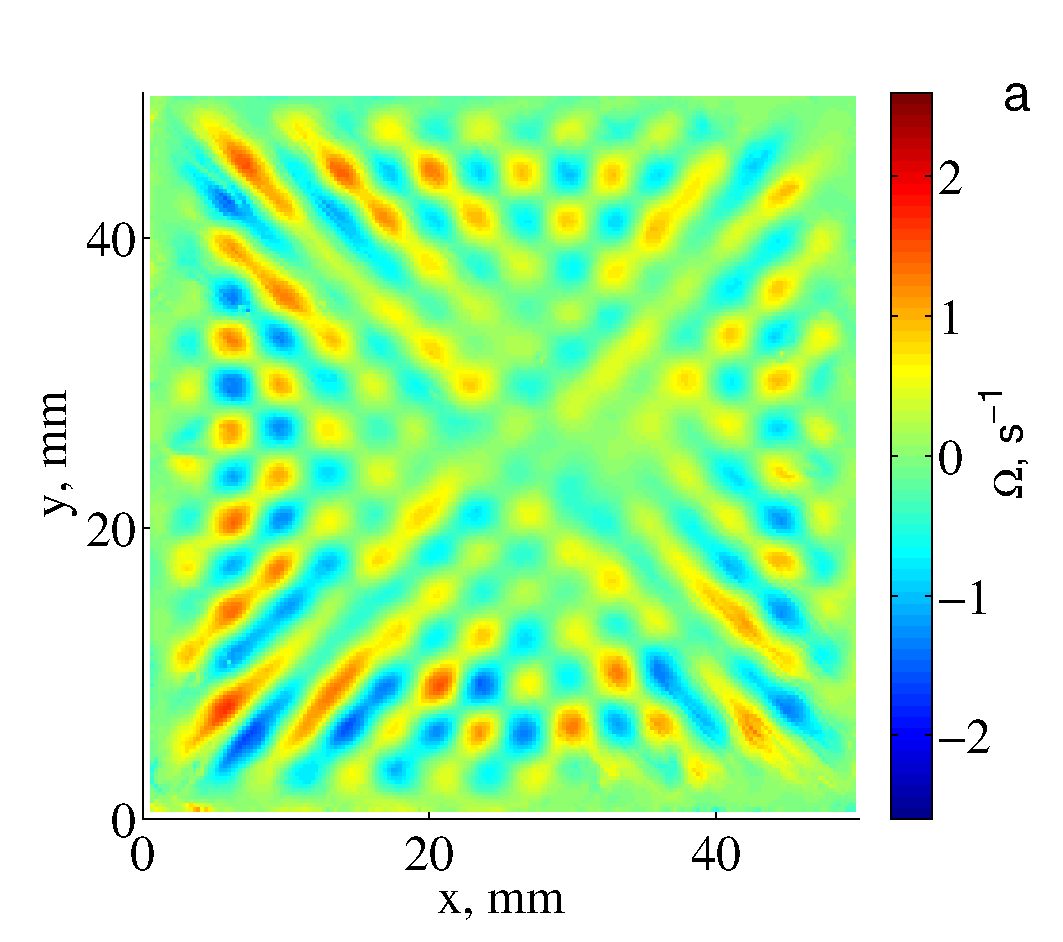
\includegraphics[width=1\linewidth]{article3/pic_03a.eps} \\ а)}
  \end{minipage}
  \hfill
  \begin{minipage}[ht]{0.49\linewidth}
    \center{\includegraphics[width=1\linewidth]{article3/pic_03b.eps} \\ б)}
  \end{minipage}
  \caption{Завихренность $\Omega$ на поверхности воды в квадратном сосуде при разных амплитудах колебаний на частоте 45.5 Гц: до порога возникновения параметрической неустойчивости (амплитуда переменного ускорения $\beta$ = 0.4, a) и после развития параметрической неустойчивости ($\beta$ = 0.48, b). Пороговое ускорение $\beta_c$ = 0.44}
  \label{img:vort_square}  
\end{figure}


На рис. \ref{img:fft_square} приведены Фурье-образы вихревых структур, представленных на рис. \ref{img:vort_square}. При накачке с амплитудой, меньшей критического значения, на поверхности доминирует структура с обратным периодом $\approx$ 10 см$^{-1}$ (рис. \ref{img:fft_square}a) в обоих направлениях, что соответствует волновому числу волны на частоте накачки. На рис. \ref{img:fft_square} б, помимо первоначальной структуры, видна структура с обратным периодом около 6 см$^{-1}$, амплитуды Фурье которой в несколько раз превышают амплитуды Фурье первоначальной структуры. Возрастание периода решетки вихрей связано с появлением на поверхности воды стоячих волн с частотой $\omega_p/2$, длина волны которых совпадает с периодом вихревой структуры, возникающей при переходе через порог неустойчивости Фарадея. 


\begin{figure}[ht]
  \begin{minipage}[ht]{0.49\linewidth}
    \center{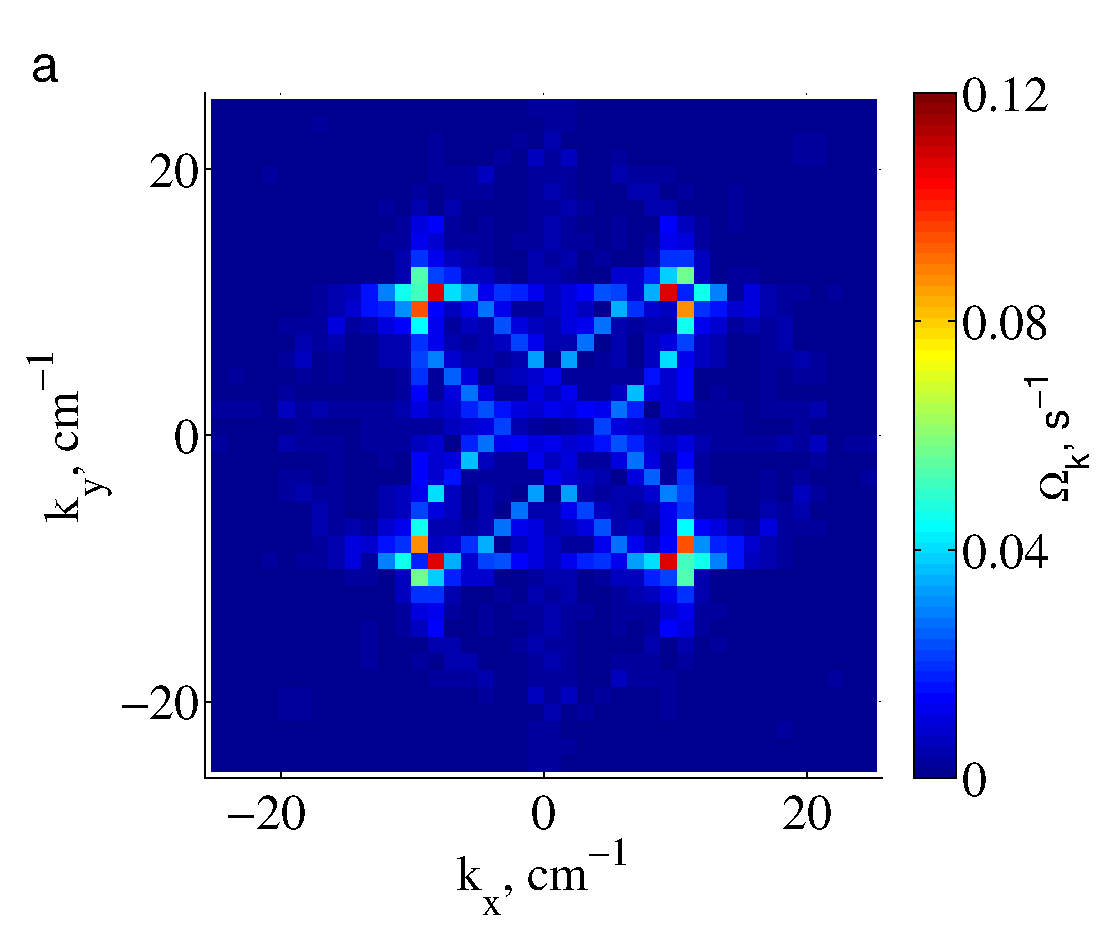
\includegraphics[width=1\linewidth]{article3/pic_04a.eps} \\ а)}
  \end{minipage}
  \hfill
  \begin{minipage}[ht]{0.49\linewidth}
    \center{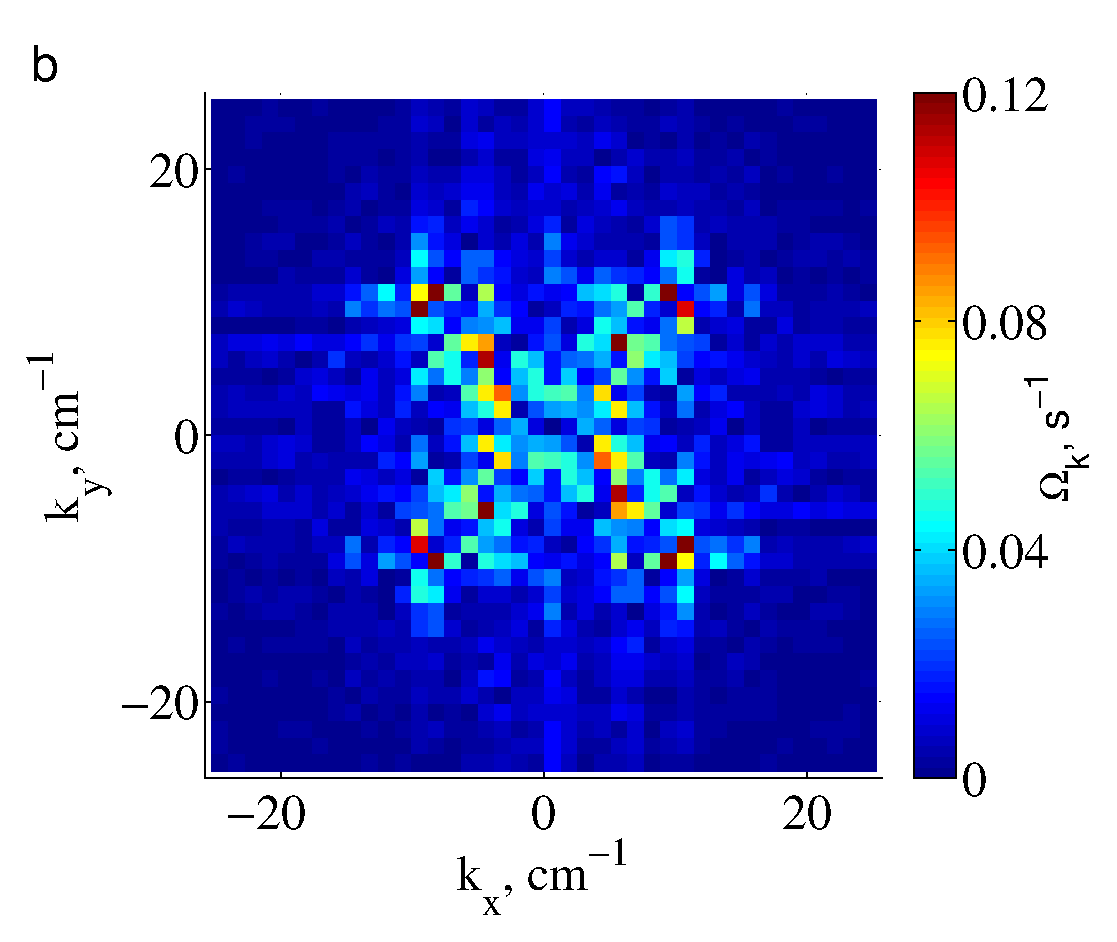
\includegraphics[width=1\linewidth]{article3/pic_04b.eps} \\ б)}
  \end{minipage}
  \caption{Фурье образ поля завихренности $\Omega_k$ на поверхности воды в квадратном сосуде при разных амплитудах колебаний на частоте 45.5 Гц: до порога возникновения параметрической неустойчивости (амплитуда переменного ускорения $\beta$ = 0.4, a) и после развития параметрической неустойчивости ($\beta$ = 0.48, б). Пороговое ускорение $\beta_c$ = 0.44}
  \label{img:fft_square}  
\end{figure}

Зависимость интегральной завихренности $|\Omega|$ движения на поверхности воды от амплитуды переменного ускорения $\beta$ в квадратном сосуде показана на рис. 5. При изменении амплитуды переменного ускорения $\beta$ от 0.11 до 0.55 модуль завихренности $|\Omega|$ возрастает почти на два порядка, причем ее быстрый рост наблюдается при ускорениях выше порога параметрической неустойчивости. При накачках ниже порогового значения изменение модуля завихренности как функции амплитуды ускорения $\beta$ хорошо описывается степенной зависимостью $|\Omega| \sim \beta^{1.7}$. Поскольку при прочих равных условиях амплитуда возбуждаемых на поверхности стоячих волн $A$ прямо пропорциональна амплитуде переменного ускорения $\beta$, зависимость интегральной завихренности от амплитуды волн будет иметь тот же показатель. Приведенная ниже оценка дает $|\Omega| \sim \beta^{2}$ \cite{F6}. Отличие, по-видимому, вызвано неоднородностью поля завихренности: вблизи края сосуда она больше, чем в центре (рис. \ref{img:vort_square}a).

\begin{figure}[ht] 
  \center
  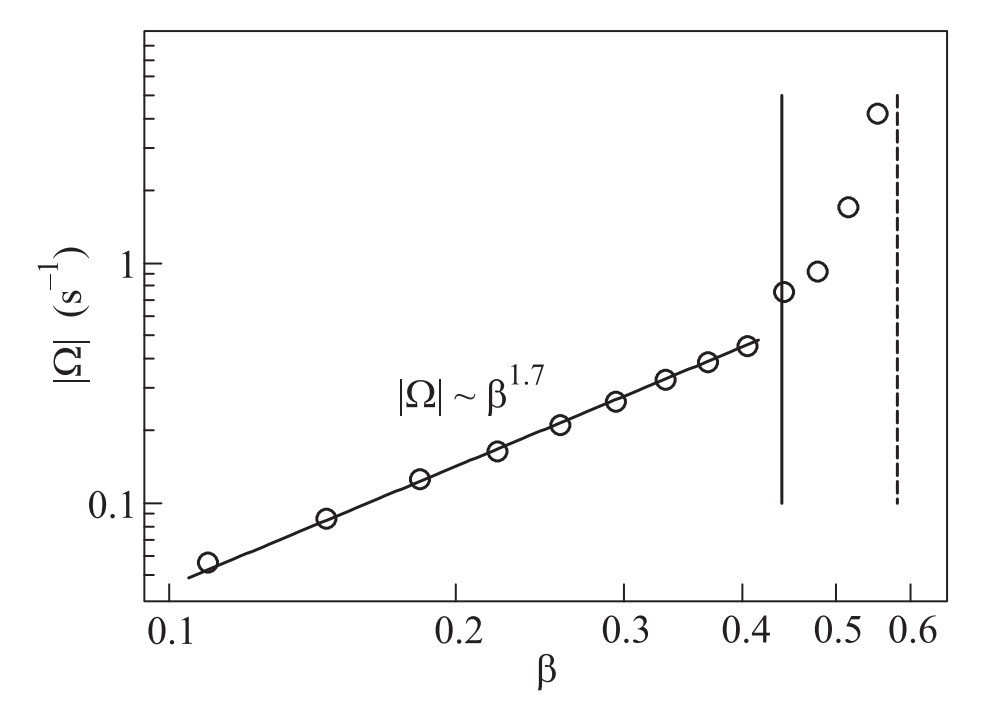
\includegraphics [scale=.4] {article3/pic12.jpg}
  \caption{Рис. 5. Зависимость суммарного модуля завихренности $| \Omega| = \int | \Omega(x,y)|dx dy$ на поверхности воды в квадратном сосуде от амплитуды переменного вертикального ускорения $\beta$. Сплошная вертикальная линия соответствует пороговой амплитуде переменного ускорения $\beta_c = 0.44$.} 
  \label{img:wave_az}  
\end{figure}

Так как в квадратном сосуде вихревое движение наблюдается при амплитудах накачки значительно ниже порога параметрической неустойчивости, формирование вихревого движения здесь не может быть приписано особенностям параметрической неустойчивости Фарадея. Тот факт, что структуры вихревого и волнового движения коррелируют между собой, позволяет предположить, что волны непосредственно участвуют в формировании вихрей. Принципиальное отличие волн в квадратном сосуде, где вихри наблюдаются, начиная с самых малых амплитуд накачки, от волн в цилиндрическом сосуде, где вихри появляются только при достижении порога неустойчивости, связано с количеством одновременно возбуждаемых мод колебаний поверхности жидкости на фиксированной частоте. В квадратном сосуде ввиду симметричности всегда возбуждается пара мод (\ref{eq:waveStand}). В цилиндрическом сосуде две разные моды, радиальная и азимутальная, одновременно возбуждаются только после превышения порога параметрической неустойчивости. Можно предположить, что изменение симметрии цилиндрического сосуда, которое приведет к возбуждению азимутальных мод при амплитудах накачки, меньших порогового значения, также сделает возможным формирование вихревого движения при этих же амплитудах.

\begin{figure}[ht]
  \begin{minipage}[ht]{0.49\linewidth}
    \center{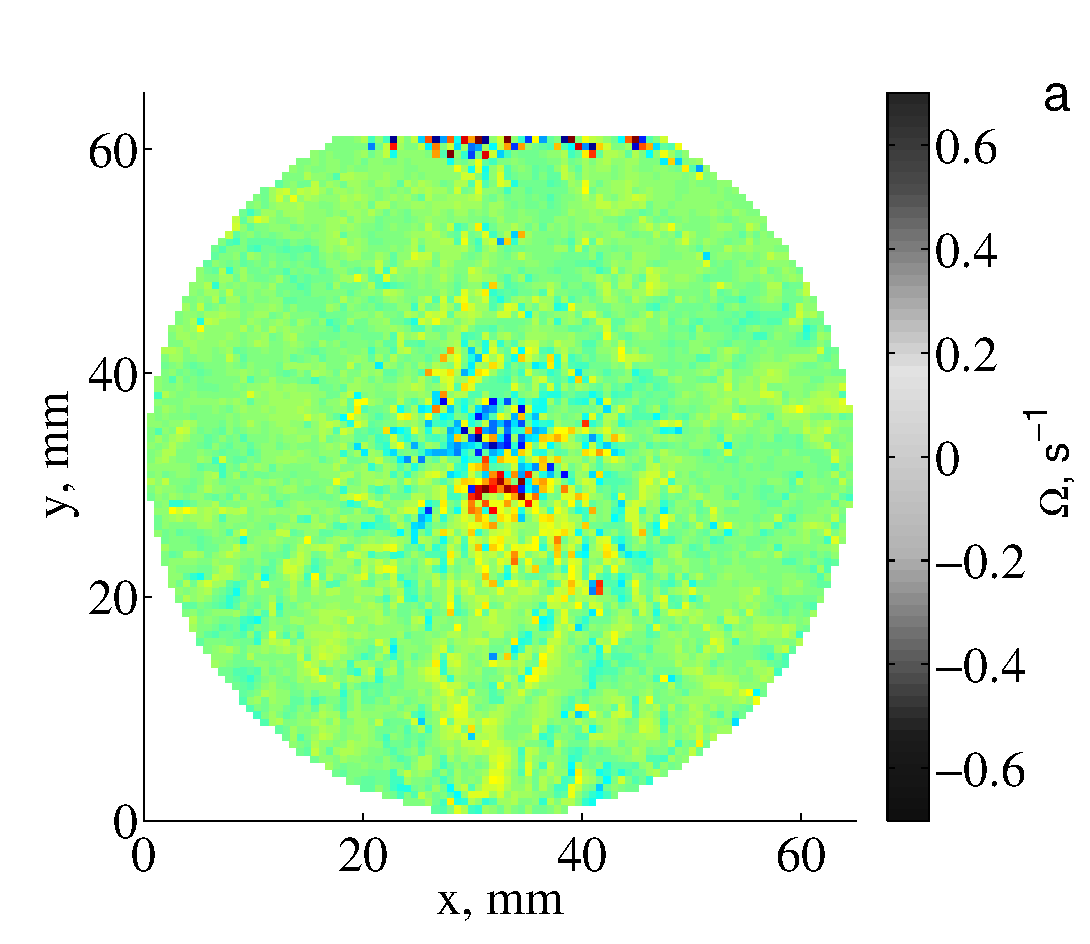
\includegraphics[width=1\linewidth]{article3/pic_06a.eps} \\ а)}
  \end{minipage}
  \hfill
  \begin{minipage}[ht]{0.49\linewidth}
    \center{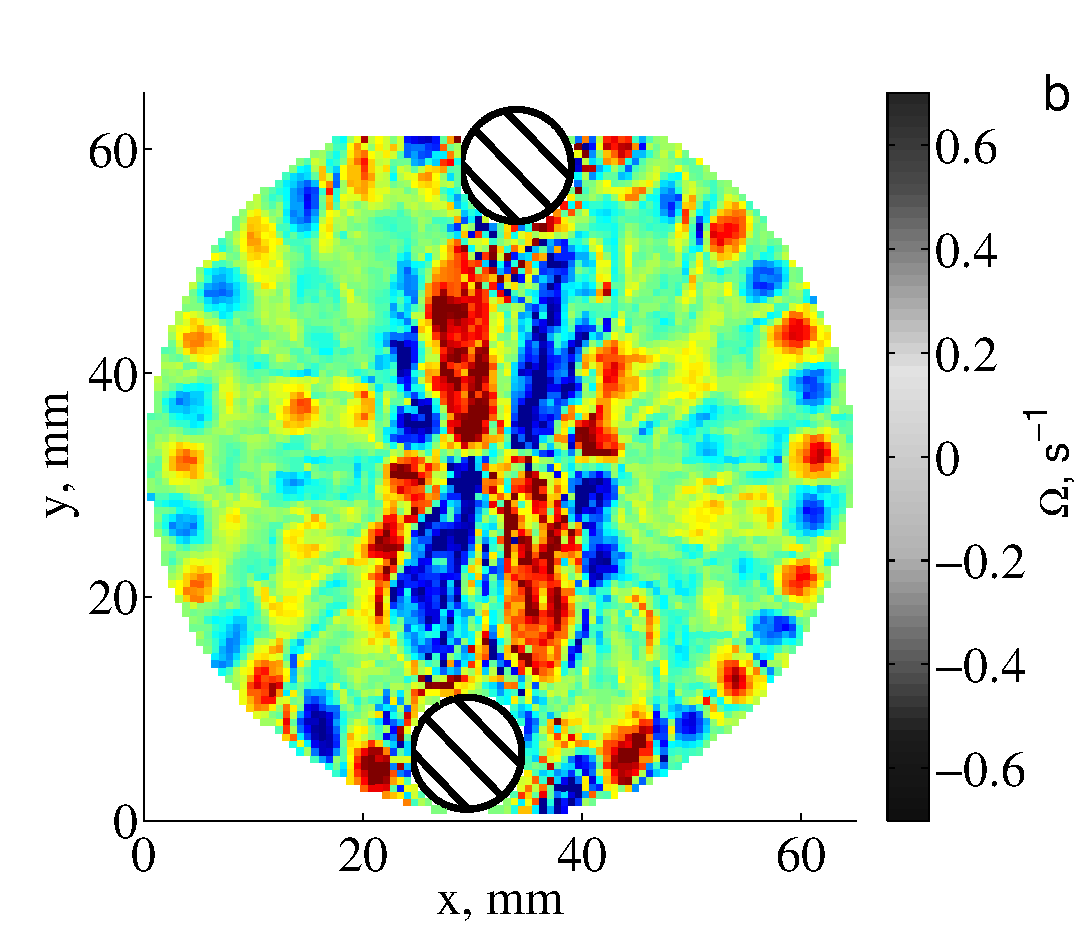
\includegraphics[width=1\linewidth]{article3/pic_06b.eps} \\ б)}
  \end{minipage}
  \caption{Поле завихренности $\Omega$ в цилиндрическом сосуде, в котором установлены два пластиковых столбика. На вставке – завихренность до установки столбиков. Цветовая шкала для завихренности общая.}
  \label{img:vort_st}  
\end{figure}

Для проверки данного предположения симметрия цилиндрического сосуда была нарушена установкой двух пластиковых столбиков диаметром 6.5 мм, размещаемых диаметрально противоположно вблизи стенки сосуда. На рис. \ref{img:vort_st} показано поле завихренности до и после установки столбиков. В сосуде без вставок на поверхности жидкости возбуждается только радиальная волна и вихревого движения не наблюдается. После установки столбиков на поверхности хорошо возбуждаются азимутальные моды и появляется серия вихрей вдоль стенки сосуда аналогично системе вихрей на рис. \ref{img:wave_az}. Поскольку обе моды возбуждаются на одной частоте, их волновые векторы должны быть близки по модулю (в пределах резонансной ширины мод) и иметь разные направления. В квадратном сосуде независимо от частоты накачки угол между волновыми векторами возбужденных волн составляет $90^\circ$. В цилиндрическом сосуде радиальную моду на большом удалении от центра сосуда можно рассматривать как плоскую волну, волновой вектор которой направлен перпендикулярно стенке сосуда. Резонансную моду с малым радиальным числом $n$ и большим азимутальным числом $m$ по аналогии с модами шепчущей галереи для акустических волн можно рассматривать как распространяющуюся вдоль границы сосуда волну. Поэтому мы полагаем, что за формирование вихревого движения здесь отвечает взаимодействие двух поверхностных волн, волновые векторы которых направлены под углом друг к другу.
%\section{Выводы} \label{sect3_3}

Таким образом было экспериментально показано, что стоячие волны на поверхности жидкости в сосуде, который совершает гармонические колебания в вертикальном направлении с амплитудой переменного ускорения ниже порога параметрической неустойчивости, могут генерировать вихревое течение. В квадратном сосуде структура вихревого движения имеет вид квадратной решетки с периодом, равным длине стоячих волн. В цилиндрическом сосуде вихревое движение наблюдается только при возникновении азимутальных мод, которые возможны при амплитудах накачки выше порога параметрической неустойчивости. Искусственное понижение симметрии цилиндрического сосуда, которое разрешает генерацию азимутальных мод при малых амплитудах накачки, позволяет формировать вихревое движение при накачке значительно ниже порога параметрической неустойчивости Фарадея. Исходя из этих наблюдений и принимая во внимание степенную зависимость завихренности от амплитуды волн, можно утверждать, что в сосудах разной симметрии вихревое движение возникает тогда, когда на поверхности жидкости распространяется пара волн с неколлинеарными волновыми векторами.

\section{Нелинейное возбуждение завихренности поверхностными волнами} \label{sect3_4}
Для описания вихревого движения формируемого волновым движение нашими соавторами по работе \cite{F6} из Института Теоретической Физики им.Л.Д. Ландау была построена теоретическая модель генерации вихревого движения нелинейно взаимодействующими волнами, распространяющимися под углом друг к другу. Подробное её описание и вывод можно найти в работах \cite{F6, Parfenyev2016}. Здесь же остановимся на выводах необходимых для интерпретации экспериментальных результатов. Для граничных условий соответствующих двум перпендикулярным стоячим волнам (см. ур-ние \ref{eq:waveStand}), было найдено приближенное распределение вертикальной составляющей завихренности по поверхности жидкости:
\begin{equation}
\label{eq:vortStand}
\Omega = -(1 + \sqrt{2})sin \phi H_1 H_2 \omega k^2 sin(kx)sin(ky).
\end{equation}
Стоит отметить, что полученный результат не зависит от времени. Так же несмотря на то, что вязкость существенна при выводе этого решение, ее нет в конечном результате. Для экспериментального изучения этого эффекта важно обратить внимание на множитель включающий разницу фазу между стоячими волнами в разных направлениях. В квадратной ячейке, разница фаз волн, возбуждаемых вертикальной тряской будет равно нулю. Поэтому для экспериментального изучения полученной теоретической модели использовалась прямоугольная ячейка размерами 49 на 50 мм$^2$. Ненулевая разница фаз будет возникать за счет различия резонансных условиях в двух перпендикулярных направлениях.
\begin{figure}[ht] 
  \center
  \includegraphics [scale=1.5] {article4/pic_01.jpg}
  \caption{Экспериментальная установка для регистрации вихревых движений на поверхности воды. а) Схема установки: 1 - ячейка, 2 - вода, 3 - виброплатформа, 4 - фотоаппарат, 5 - фотовспышка. b) Вогнутый или выпуклый мениск формируется на краю стенок в зависимости от количества воды, используемой для заполнения сосуда. с) Конфигурация водяного мениска в квадратной ячейке, имеющей стенки разной высоты, предназначенная для подавления генерации волн от пары соседних стенок. Стрелки показывают направление распространения волны.} 
  
  \label{img:setup50}  
\end{figure}
Для проверки теоретических предсказаний использовались две ячейки различной геометрии, показанные на рис. \ref{img:setup50}. В ячейке размерами 49 на 50 мм (рис. \ref{img:setup50} б) стенки имеют одинаковую высоту, поэтому на поверхности жидкости устанавливаются стоячие волны. В то время как у ячейки, показанной на рис. \ref{img:setup50} с противоположные стенки имеют разную высоту. Форма мениска у противоположных стенок будет так же отличаться. Меняя уровень воды можно добиться того, что на поверхности воды будут возбуждаться бегущие волн вместо стоячих.
%  Конфигурация водяного мениска в квадратной ячейке, которая имеет стенки разной высоты, предназначенные для подавления генерации волн от пары соседних стенок. Стрелки показывают направление распространения волны.
Стационарная картина стоячих капиллярных волн формируется в течении 1-2 с после включения возбуждения. Одновременно с рябью возникает квадратная решетка вихрей на поверхности. Вся картина остается стабильной по крайней мере в течение нескольких минут. Результаты эксперимента представлены на рис. \ref{img:vort_chess} и \ref{img:vort_roll}, где показана завихренность $\varpi_z$ усредненная по времени. Красный цвет соответствует положительной завихренности, синий цвет - отрицательной завихренности, цветовая шкала определяющая значение завихренности так же представлена на рисунке справа.

\begin{figure}[ht] 
  \center
  \includegraphics [scale=.7] {article4/pic_02.eps}
  \caption{Завихренность в ячейке 50 x 49 мм$^2$ при возбуждении поверхностных волн с частотой 42.7 Гц. Наблюдается шахматноподобный паттерн поля завихренности соответствующий теоретическому выражению (14). Периоды решетки в $X$ и $Y$ направлениях равны длине волны.} 
  \label{img:vort_chess}  
\end{figure}

\begin{figure}[ht] 
  \center
  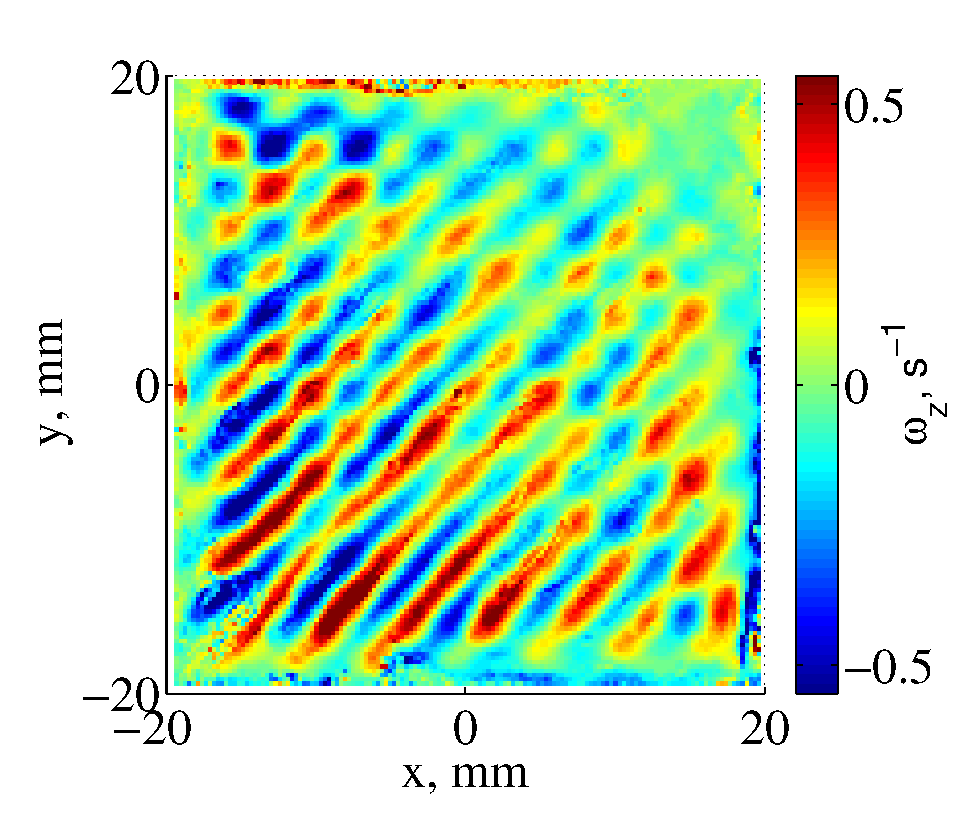
\includegraphics [scale=.7] {article4/pic_03.eps}
  \caption{Завихренность в ячейке 40 х 40 мм $^2$ при возбуждении поверхностных волн с частотой 54 Гц. Две стенки ячейки соответствующие левой и нижней части рисунка немного ниже, чем остальные станки. Уровень воды скорректирован, чтобы в основном возникало две бегущие волны от более низких стенок. Знакопеременные полосы положительной и отрицательной завихренности, направленные параллельно диагонали квадратной ячейки, согласуются с теоретическим выражением (16).} 
  \label{img:vort_roll}  
\end{figure}


Для объяснения результатов сначала заметим, что волны возбуждающиеся мениском воды, сформированным около стенок. Следовательно, действующие силы локализованы около стен и можно использовать свободные гидродинамические уравнения для описания движения воды не очень близко к стенам. Мы имеем дело с почти линейными волнами заданной частоты, амплитуда волн определяется пристенными силами и граничными условиями. В ячейке возникают только волны распространяющиеся перпендикулярно от стенок прямоугольной ячейки. Резонансные частоты соответствуют волнам с длиной волны соответствующей граничному условию: длина стенок ячейки равна целому числу длин волн с точностью до некоторой поправки, связанной с пристеночной областью. Линейный размер сосуда достаточен, чтобы расстояние в частотном пространстве между соседними резонансами было больше, чем ширина резонансов. Волны распространяющиеся в других направлениях не возбуждаются, так как мощность передаваемая от мениска волне в этом случае пренебрежимо мала.

На рисунке \ref{img:vort_chess} показана завихренность наблюдаемая в почти квадратной ячейке, где стоячие волны возбуждаются в $X$ и $Y$ направлениях.

% Пренебрегая затуханием волн, мы можем моделировать высоту жидкости как:
%
%\begin{equation}
% %\label{eq:disperCap}
%h = H_1 cos(\omega t) cos(kx) + H_2 cos(\omega t + \phi) cos(ky),
%\end{equation}
%где $k$ определяется законом дисперсии. Фазовый сдвиг $\phi$ в уравнении (13) возникает из асимметрии ячейки, которая приводит к разным граничным условиям для стоячих волн в $X$ и $Y$ направлениях. Изменяя соотношение сторон ячейки можно менять разность фаз $\phi$. Подставляя выражение (13) в уравнение (12) получаем:


%Этот результат не зависит от времени. Сумма рациональных и иррациональных чисел соответствует сумме двух слагаемых в уравнении (12), которые имеют различную глубину проникновения. Это выражение (14) качественно соответствует рисунку \ref{img:vort_chess}.

Мы также проводили эксперименты с квадратной ячейкой, где разница фаз $\phi \ll 1$ (см. рис. \ref{img:vort_square}). Видно что распределение завихренности на рис. \ref{img:vort_square} и \ref{img:vort_chess} существенно отличаются. Для описания распреденения завихренности на поверхности следует учитывать затухание волны вдоль направления распространения волны из-за вязкого затухания. %Детали представлены в Дополнительной материала [7].

Амплитуда завихренности как функция амплитуды волны показана на рисунке \ref{img:vort_ampl}. Высота отклонения поверхности вызванная волнами была измерена лазерным лучом отраженным от жидкой поверхности. Размер лазерной проекции на экран может быть пересчитан в амплитуду наклона поверхности $kH$, где $H$ амплитуда наибольшей волны. График на рисунке \ref{img:vort_ampl} показывает квадратичную зависимость завихренности от угловой амплитуды волны, что соответствует нашим теоретическим предсказаниям.

\begin{figure}[ht] 
  \center
  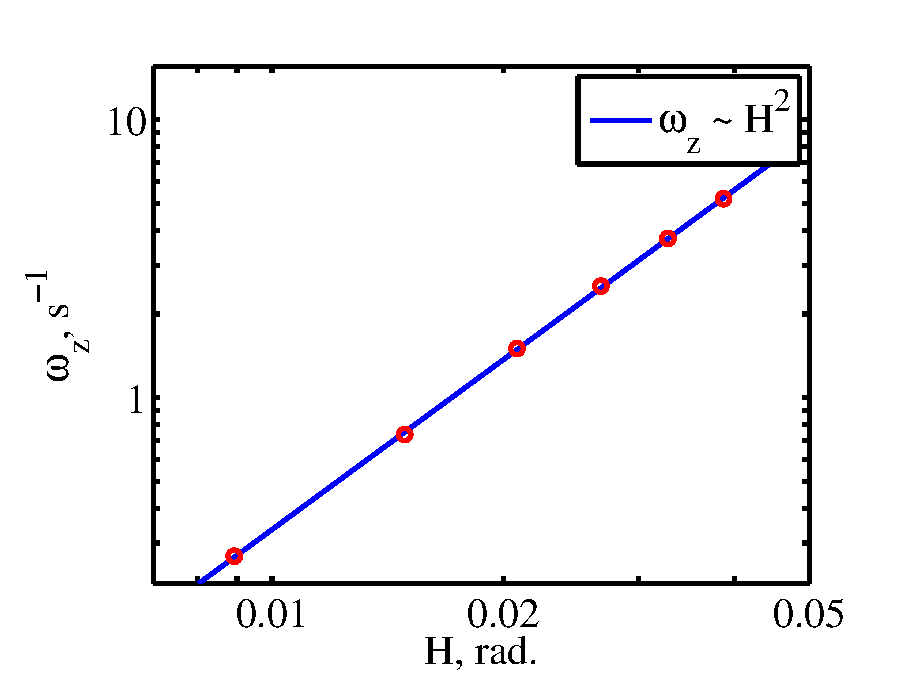
\includegraphics [scale=.7] {article4/pic_04.eps}
  \caption{Амплитуда завихренности для различных амплитуд накачки в ячейке 50 x 49 мм$^2$, где возбуждаются поверхностные волны с частотой 42.7 Гц, строится в зависимости от амплитуды наклона $kH$. Линия соответствует зависимости $\Omega \sim kH^2$.} 
  \label{img:vort_ampl}  
\end{figure}

На рисуноке \ref{img:vort_roll} представлены результат другого эксперимента. В этом эксперименте квадратная ячейка имела стенки разной высоты: две смежные стенки немного ниже, чем две противоположные стенки (см. рис. \ref{img:setup50}). Для устранения мениска ячейка была наполнена водой точно по край высоких стенок. На низких стенках вода образует выпуклый мениск(см рис \ref{img:setup50}с). Таким образом возбуждающие силы приложены исключительно на низких стенках. Пренебрегая эффектом отраженных волн, можно получить грубую модель распространяющихся от низких стенок волн. Тогда отклонение поверхности будет задано как:

\begin{equation}
 \label{eq:vortRun}
h = H_1 cos(\omega t - kx) + H_2 cos(\omega t - ky),
\end{equation}

А уравнение описывающее поле завихренности согласно построенной теоретической модели выглядит как:

\begin{equation}
 \label{eq:OmegaRun}
\Omega = -(1 + \sqrt{2})sin \phi H_1 H_2 \omega k^2 sin(kx-ky).
\end{equation}
Заметим, что результат так же не зависит от времени. Рисунок \ref{img:vort_roll} показывает, что пространственное затухание волн сказывается на распределении завихренности. Учет затухания корректирует выражение (\ref{eq:OmegaRun}), что приводит к разумному качественному согласию между экспериментальными данными и теоретическими предсказаниями.% [7]. 

\section{Выводы}
Открыт новый механизм генерации поверхностной завихренности связанный с взаимодействием нелинейных поверхностных волн в тонком вязким подслоем. 
%В частности этот механизм приводит к перемешиванию поверхности, которое может быть характерезовано как диффуззионным коэффициентом $D$ соответсующиего четвертому порядку волновой амплитуды, так из прямым действием волн на поверхности жидкости \cite{Falkovich2009, Buhler}. Однако данная задача требует дальнейшего исследования.
Экспериментально наблюдена квадратичная зависимость модуля завихренности от угловой амплитуды волны.
%полученная квадратичная зависимость завихренности от амплитуды волн подтверждает нелинейность данного эффекта.
Наблюденные экспериментальные распределения вихревого движения, генерируемого взаимно перпендикулярными как стоячими, так и бегущими волнами, качественно хорошо согласуются с теоретической моделью.
 %Несмотря на то, что эксперименты производились в капиллярной области, приведенные теоретические построения также применимы и в на гравитационной области. Для примера соответствующая теория может быть использована для анализа вихревого движения на поверхности океана.

Увеличивая амплитуду вертикальных колебаний ячейки можно достичь порога неустойчивости Фарадея. Значительно выше порога, поверхностные волны весьма интенсивны, что приводит к интенсивным вихревым движениям поверхности жидкости, для которых угловая амплитуда приближается к 1. Тогда взаимодействие вихревых движений друг с другом становится значительным \cite{Punzmann}, что приводит, в частности, к образованию каскада энергии \cite{Francois2013}. Результаты наших теоретических и экспериментальных исследований позволяют лучше понять это явление и разработать количественную основу для него.

\clearpage